\documentclass[a4paper,12pt]{article} % тип документа
\usepackage[margin=1in]{geometry} % Поля

%  Русский язык
\usepackage[warn]{mathtext}
\usepackage[T2A]{fontenc}			% кодировка
\usepackage[utf8]{inputenc}			% кодировка исходного текста
\usepackage[english,russian]{babel}	% локализация и переносы
% Математика
\usepackage{amsmath,amsfonts,amssymb,amsthm,mathtools} 
\usepackage{wasysym}
%%%
\usepackage{graphicx}

\usepackage{tabularx}

\usepackage{gensymb} % знак градуса
\usepackage{enumitem} % изменить список enumerate
\usepackage{placeins} % \FloatBarrier

\renewcommand{\thesection}{\Roman{section}} 
\renewcommand{\thesubsection}{\roman{subsection}}



\begin{document}

\newcolumntype{Y}{>{\centering\arraybackslash}X} %new tabularx


%титул
\hrule 	
\medskip
\begin{raggedright}
{\large \textbf{Отчёт по лабораторной работе № 18}}
\\
\medskip
{\Large Вибрационный магнитометр} 
\\
\medskip
{\large Карташов Констанин Б04-005}
\medskip
\hrule
\medskip
\end{raggedright}


\section{Теоретическая часть}

\paragraph{}
	В настоящее время в качестве устройств для измерения магнитного момента получили распространение магнитометры с вибрирующим образцом (вибромагнитометры). Суть метода заключается в следующем: образец намагничивается постоянным магнитным полем в зазоре электромагнита и одновременно приводится в периодическое движение с низкой частотой. Поля рассеяния, обусловленные намагниченностью вибрирующего образца, создают осциллирующий магнитный поток в расположенный поблизости измерительной катушке. Согласно явлению электромагнитной индукции в катушке возникает переменное напряжения (ЭДС индукции), которое и является мерой намагниченности вещества (сравнивается с ЭДС от эталонного образца)

\begin{figure}[h]
\centering
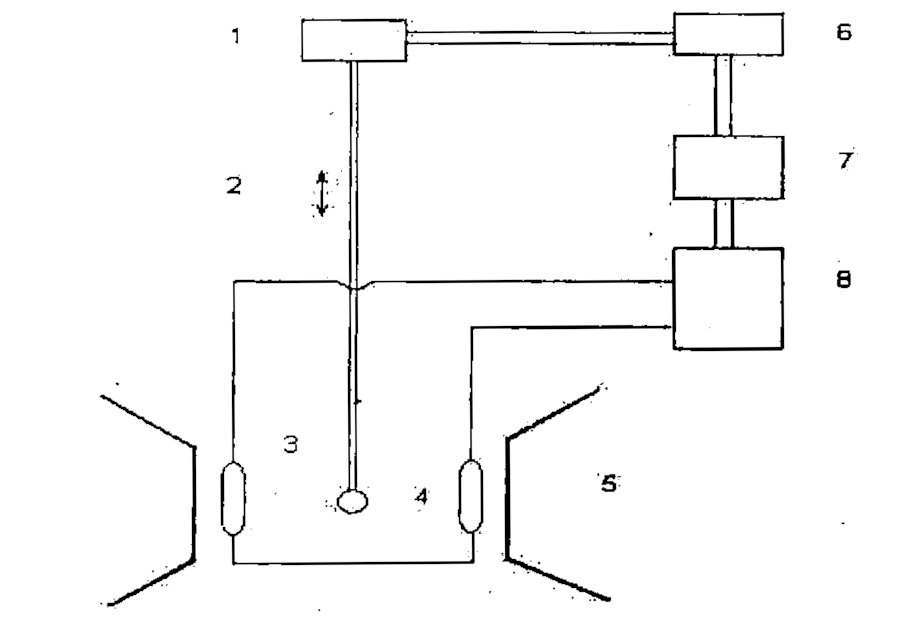
\includegraphics[width=0.5\textwidth]{setup.png}
\caption{Блок-схема вибомгнитометра: 1 -- вибропреобразователь, 2 -- шток, 3 -- образец, 4 -- приёмные катушки, 5 -- электромагнит, 6 -- генератор, 7 -- синхронный детектор, 8 -- узкополосный усилитель}
\label{fig:setup}
\end{figure}


\paragraph{}
	Блок-схема вибромагнитометра представленная на рисунке \ref{fig:setup}. Принцип работы заключается в следующем: вибропреобразователь (1), питаемый от генератора синусоидального тока (6), приводит в поступательной периодическое движение шток (2) с образцом (3). Образец находится под воздействием постоянного намагничивающего поля от электромагнита (5). В результате в приёмных катушках (4) наводится ЭДС индукции. Образовавшееся напряжение поступает на вход селетивного усилителя (8), а с выхода усиленный сигнал поступает на вход синхронного детектора (7), при этом на другой вход детектора поступает сигнал с генератора (6). В результате на выходе детектора (7) образуется постоянный по амплитуде сигнал, пропорциональный амплитуде ЭДС индукции, а следовательно, и величине магнитного момента образца (3). Таким образом, осуществятся на практике принцип синхронного детектирования. 
	
\paragraph{}
	Математически принцип электромагнитной индукции описывает на основе закона Био-Савара: \[ \mathcal{E} = - \frac{d\Phi}{dt}. \] Здесь $\mathcal{E}$ -- ЭДС индукции, $\Phi$ -- магнитный поток. При этом $\Phi = BSn$, $B$ -- индукция, $S$ -- площадь витка, $n$ -- количество витков. Для небольших по амплитуде колебаний штока имеет место следующее соотношение: $\Delta B \propto A \sin(\omega t)$, где $\Delta B$ -- разность в величине индукции по площади вика при крайних положениях штока, $A$ -- амплитуда колебаний штока, $\omega$ -- частота колебаний. Тогда $\mathcal{E} \propto -nSA \omega \sin(\omega t)$.

	

\medskip\hrule\medskip

\section{Экспериментальная часть}

\paragraph{} Поместим образец на экспериментальную установку (уже был установлен). Включим блок постоянного тока, генератор переменного напряжения, синхронный детектор. Проверим работу синхронного детектора: после подачи опорного и входного сигналов на приборной панели должны выключится красный индикатор отсутствия синхронизации и должно появится показание пропорциональное амплитуде чистого сигнала.

\paragraph{} Найдём оптимальный режим работы экспериментальной установки. Для этого подадим на катушку постоянный ток $I = 0.83$ А и будем менять частоту переменного сигнала, при этом фиксируя показания синхронного детектора. Так как показания синхронного детектора пропорциональны амплитуде полезного сигнала, при максимальных показаниях синхронного детектора амплитуда полезного сигнала будет максимальной. Полученная зависимость показана на рисунке \ref{fig:plot_1}. Из этого можем сделать вывод что оптимальная частота колебаний $f_\text{опт} \approx 35$ Гц.

\begin{figure}[h]
\centering
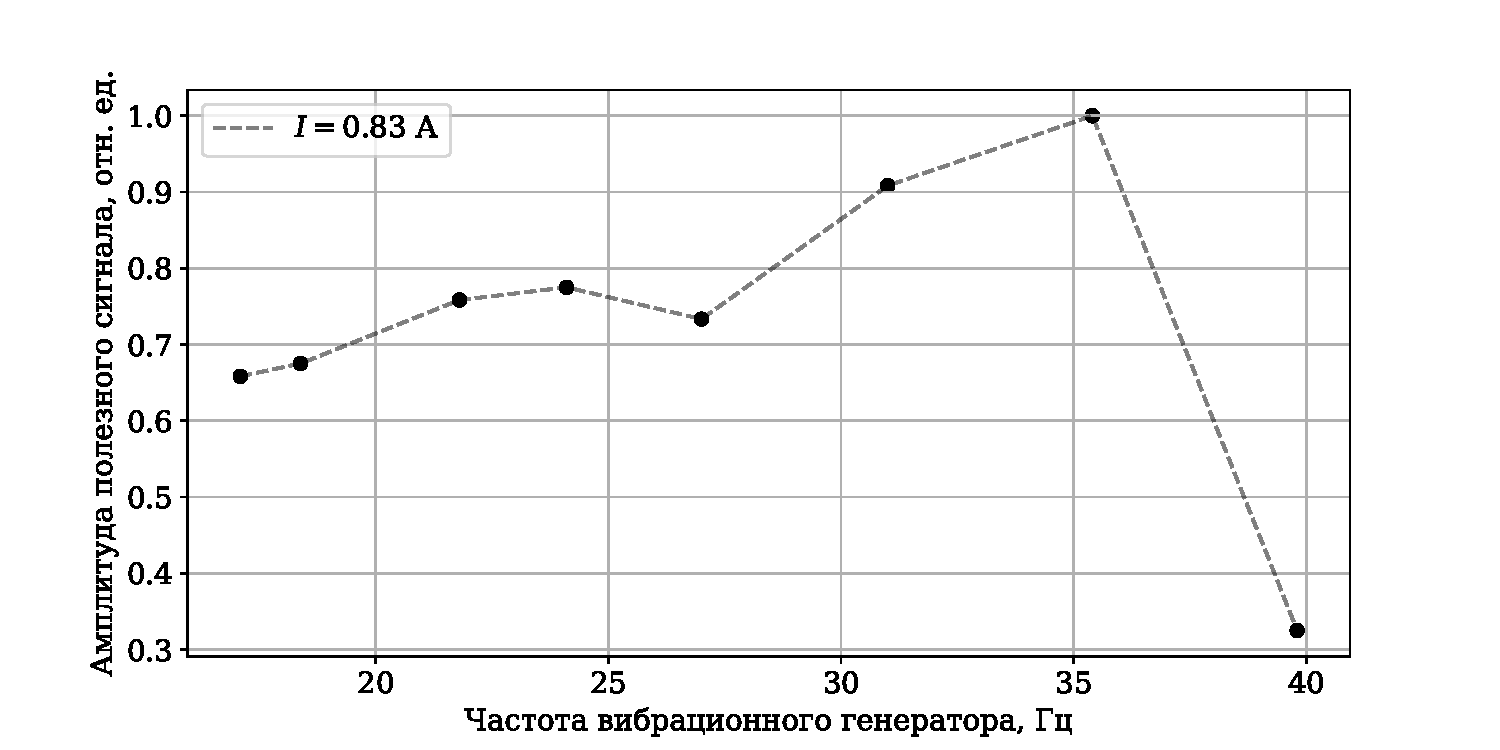
\includegraphics[width=\textwidth]{plot_1.pdf}
\caption{Зависимость амплитуды полезного сигнала от частоты колебаний установки.}
\label{fig:plot_1}
\end{figure}

\paragraph{} Найдём зависимость намагниченности образца от величины магнитного поля создаваемого катушкой. Для этого выставим частоту колебаний равной найденной оптимальной частоте. И снимем зависимость показаний синхронного детектора от величины тока в катушке. Так как ток в катушке пропорционален напряжённости постоянного магнитного поля создаваемой ей, а показания синхронного детектора пропорциональны намагниченности образца, полученная зависимость будет пропорциональна искомой зависимости. Полученная зависимость показана на рисунке \ref{fig:plot_2}.

\begin{figure}[h]
\centering
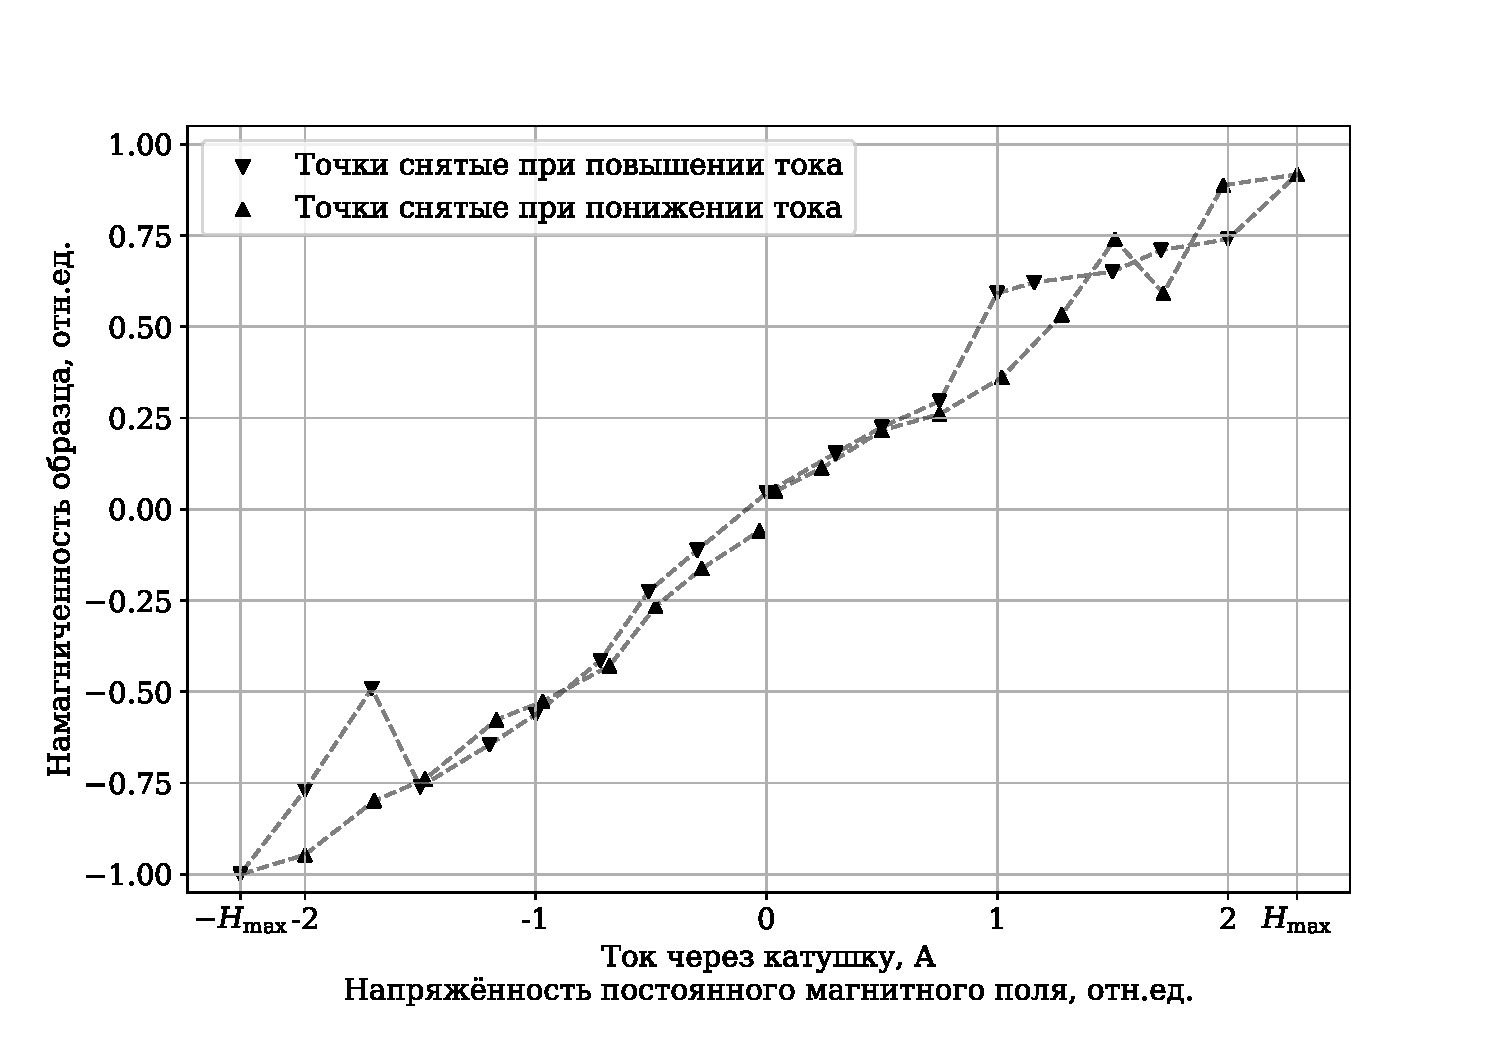
\includegraphics[width=\textwidth]{plot_2.pdf}
\caption{\centering Зависимость намагниченности образца от напряжённости постоянного магнитного поля}
\label{fig:plot_2}
\end{figure}


\medskip\hrule\medskip

\section{Выводы}

\begin{enumerate}
\item Изучили принцип работы вибрационного магнитометра и показали применимость метода на практике.
\item Нашли оптимальный режим работы вибрационного магнитометра при помощи синхронного детектора.
\item Изучили зависимость намагниченности образца от напряжённости постоянного магнитного поля катушки при помощи синхронного детектора. Так как зависимость показала отсутствие остаточной намагниченности, можно сделать вывод, что образец парамагнетический, либо напряжённости магнитного поля недостаточно для появления остаточной намагниченности.
\end{enumerate}

\medskip\hrule\medskip

\end{document}
